% \newpage
\section{Case Study}



% Based on Hingoranoi-Kohler 2023 Sustainability potential of risk-informed decisions in structural design:

% Beam with cost, emission functions, adjust to my approach.

% Pick handful of representative cases (2-3).

% Show 2-objective first, Pareto front. Then single-objective, linked by shadow price.

% Variation study? Focus on damage costs, emission intensity. Cobweb plots?

The proposed augmented framework is demonstrated in this section using a typical structural design problem: a simply supported steel beam in an office building, see Figure \ref{fig:beam}.
This case study is adapted from previous work by Hingorani and Köhler \citep{Hingorani2023SustainabilityDesign, Hingorani2023TowardsDesign} where the design of a beam carrying a hollow-core slab floor in an office building was optimised separately for costs and emissions.
The previous paper by the authors presented a similar case study for determining acceptable reliability while taking emissions into account \citep{Knibbe2026PlaceHolder}.

The decision parameter $x$ in this case study represents the plastic section modulus of the beam (in $[mm^3]$), setting its bending moment resistance.
The corresponding limit state function is:

\begin{equation}
    \label{eqn:LSF}
    Z = \theta_R f_y x - \theta_E \frac{(g_{sw} + g_{nsl} + \theta_q q_{live})DL^2}{8}
\end{equation}

Where the beam yield strength $f_y$, loads $g_{sw}$, $g_{nsl}$ and $q_{live}$ and model uncertainties $\theta_R$, $\theta_E$ and $\theta_q$ are stochastic variables.
Their distributions are derived based on the JCSS probabilistic model code \citep{JCSS2000ProbabilisticDesign}, the reliability background of the Eurocodes \citep{Vrouwenvelder2024ReliabilityEurocodes}, and \citep{Hingorani2023TowardsDesign}.
They are described in Table \ref{tab:distributions}.
The beam length $L$ and beam spacing $D$ are deterministic and set at 12 m.
Figure \ref{fig:P_f} shows how $P_f$ varies with the section modulus $x$.

\begin{figure}
    \centering
    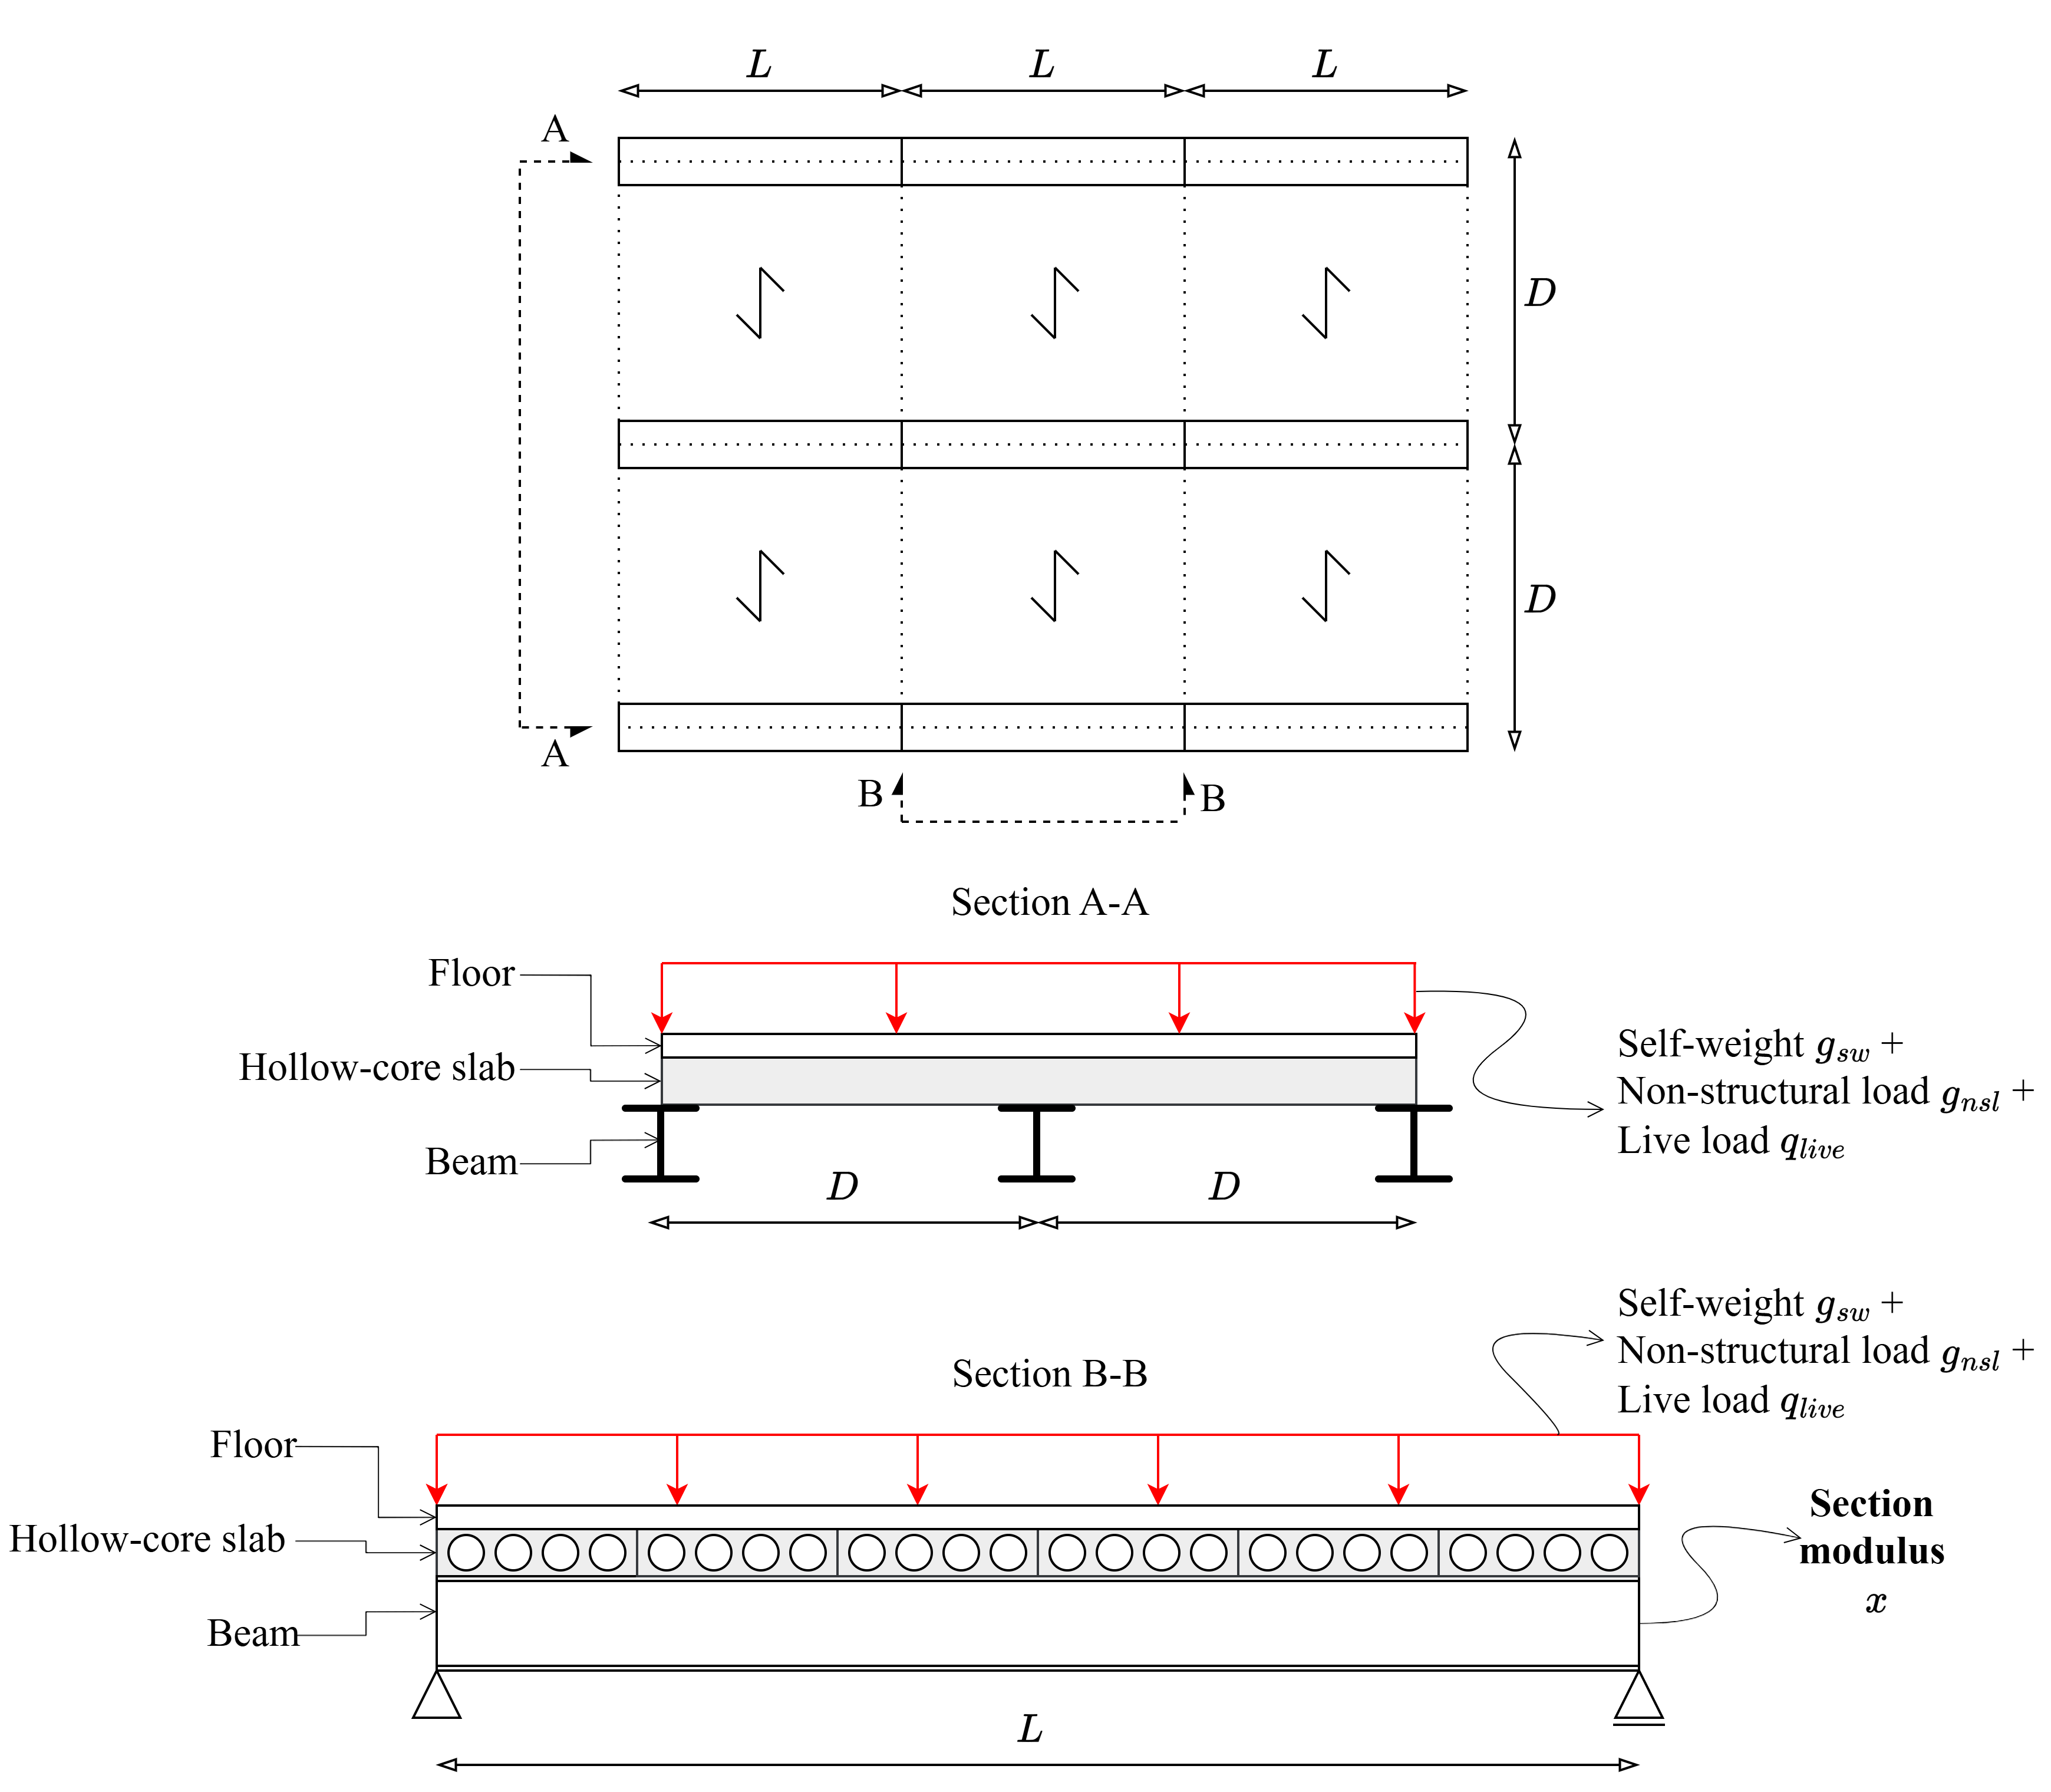
\includegraphics[width=0.8\linewidth]{Images/beam_diagram.png}
    \caption{The typical case study, with the loads, dimensions and decision variable indicated. Not to scale.}
    \label{fig:beam}
\end{figure}

\begin{table}[h]
    \centering
    
    \begin{tabular}{c|c|c|c|c|c}
         Variable & Description & Unit & Distribution & Mean & CoV  \\ \hline
         $q_{live}$& Variable load & kN/m\textsuperscript{2}& Gumbel & 1.2&0.5\\
         $g_{sw}$& Self-weight load& kN/m\textsuperscript{2}& Normal& 4.137& 0.1\\
         $g_{nsl}$& Non-structural load& kN/m\textsuperscript{2}& Normal& 2.8&0.1\\
         $f_y$& Yield strength steel& N/mm\textsuperscript{2}& Lognormal& 282&0.05\\
         $\theta_R$& Resistance model uncertainty&-& Lognormal& 1.225&0.075\\
         $\theta_E$& Load effect model uncertainty&-& Lognormal& 1.0&0.1\\
         $\theta_q$& Live load model uncertainty&-& Lognormal& 1.0&0.1\\
         $L$ & Beam length & m & Deterministic & 12 & - \\
         $D$ & Beam spacing & m & Deterministic & 12 & - \\
         $x$ & Plastic section modulus & mm\textsuperscript{3} & Deterministic & \emph{To be optimised} & - \\
    \end{tabular}
   \caption{Distributions of random variables in the limit state function used in the case study, derived from \citep{Vrouwenvelder2024ReliabilityEurocodes,Hingorani2023TowardsDesign}.} \label{tab:distributions}
\end{table}

\begin{figure}[h]
    \centering
    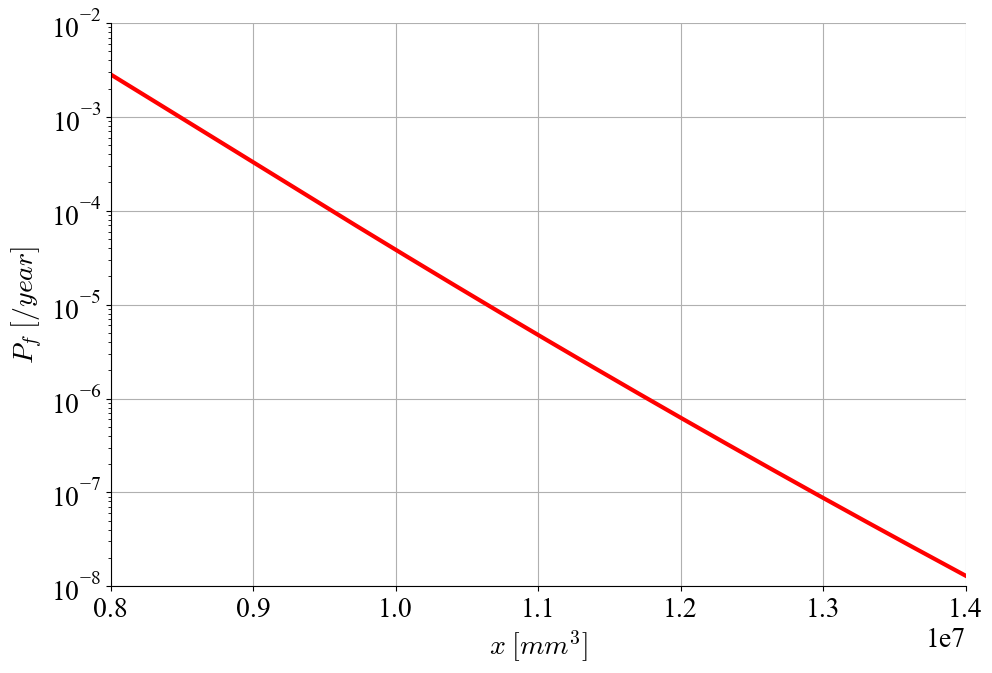
\includegraphics[width=0.7\linewidth]{Images/P_f.png}
    \caption{Failure probability $P_f(x)$}
    \label{fig:P_f}
\end{figure}

The linear formulation for the construction cost and emissions is used, with parameters given in Table \ref{tab:C_E_params}.
The $x$-independent costs $C_0$ and emissions $E_0$ are estimated on indications of labour costs and transport emissions \citep{Knibbe2026PlaceHolder, Musa2024COPeriod, Fortus2025StalenVergunning}.
The values for $C_1$ and $E_1$ are based on an assumed linear relation between the beam mass and section modulus, given in \citep{Hingorani2023SustainabilityDesign}, along with a steel material cost of 2 \EUR{}/kg steel \citep{Hingorani2023SustainabilityDesign, bauforumstahle.V.2026BaukostenBauforumstahl} and emission intensity 1.87 kg CO\textsubscript{2}eq/kg  steel \citep{TATASteel2017BenefitsOwnership}.
As mentioned in Section \ref{sec:appraisal}, using $SWTP \cdot N_f$ as (part of) the additional damage costs $C_H$ is justified. 
In this case, it is assumed that $C_{H,other}$ is negligible compared to this term. 
The number of expected fatalities in the case of failure is estimated at 0.97 \citep{Knibbe2026PlaceHolder, Hingorani2020ConsequenceStructures}, with the SWTP equal to 2.775 million \EUR{} per life saved, resulting in a $C_H$ of 2.70 million \EUR{}.
Finally, the additional failure emissions $E_H$ are derived from the loads carried by the beam, representing the embodied emissions of the floor and other, non-structural components which are replaced in the case of failure \citep{Knibbe2026PlaceHolder, Hingorani2023SustainabilityDesign}.

\begin{table}[]
    \centering
    \begin{tabular}{c|c|c|c}
         Parameter & Description& unit  &value 
\\ \hline
 $C_0$& $x$-independent costs& EUR  &1.00*10\textsuperscript{3} 
\\
 $C_1$& $x$-dependent costs&EUR$/mm^3$ &9.81*10\textsuperscript{-4}
\\
 $C_H$& Additional failure costs&EUR &2.70*10\textsuperscript{6}
\\
 $E_0$& $x$-independent emissions&kg CO\textsubscript{2}eq &3.33*10\textsuperscript{2}
\\
 $E_1$& $x$-dependent emissions&kg CO\textsubscript{2}eq/$mm^3$ &9.17*10\textsuperscript{-4}
\\
 $E_H$& Additional failure emissions&kg CO\textsubscript{2}eq &6.65*10\textsuperscript{4}\\\end{tabular}
    \caption{Parameter values in the cost and emission functions}
    \label{tab:C_E_params}
\end{table}

To find an optimal reliability, several different optimisations are now performed.
First, the cost and emission functions are considered as two separate optimisations, before being combined in a multi-objective optimisation problem.
Next, the primary weighted sum approach is presented, combining the costs and emissions in one objective function.
Finally, the alternative $\varepsilon$-constraint is considered, considering one of the functions as a constraint.

\subsection{Separate objectives}

In this approach, both objective functions are optimised separately.
The result is two optimal values for the design parameter $x$, denoted here as $x_{opt,C}$ and $x_{opt,E}$, and accompanying $\beta_{opt,C}$ and $\beta_{opt,E}$.
Figure \ref{fig:separate} and Table \ref{tab:separate} show the results of this approach.
Both functions have a similar shape, with the optimum of $C_{total}$ located at a larger value of $x$ compared to the optimum of $E_{total}$ (marked by a blue and green star, respectively), making $\beta_{opt,E}$ smaller than $\beta_{opt,C}$ ($P_{f,opt}$ is larger). 
This is caused by the difference in the `push-pull' effect between the two objectives.
The ratio $E_H/E_1$ is smaller for the emissions compared to the equivalent ratio $C_H/C_1$ for the costs, so the optimal failure probability considering emissions is `pushed' upwards relative to the cost-optimal failure probability, which has a stronger `pull' downwards.
In the next steps, values between the two optima will be considered.

\begin{figure}[h!]
    \centering
    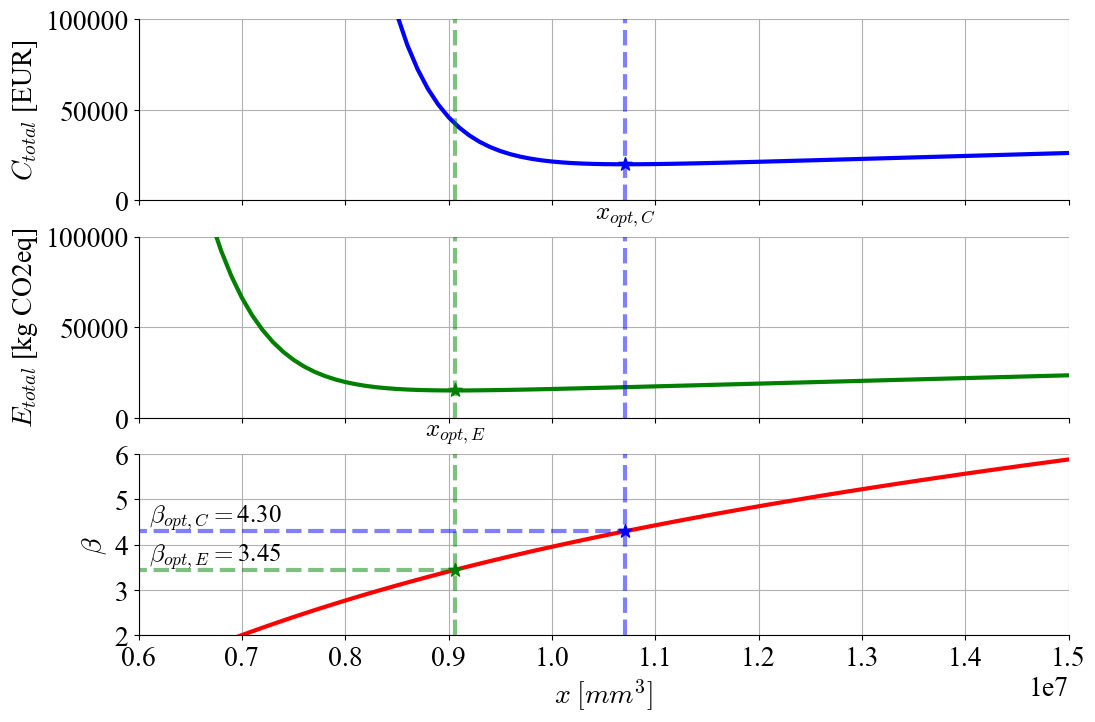
\includegraphics[width=0.95\textwidth]{Images/demo_separate.png}
    \caption{Separate optimisation of the two costs and emissions.}
    \label{fig:separate}
\end{figure}



\begin{table}[h]
    \centering
    \begin{tabular}{c|c|c|c}
         &   $C_{tot}$ optimal&$E_{tot}$ optimal &Unit\\ \hline
         $x_{opt}$& 
     $1.07*10^7$&$9.06*10^6$ &mm\textsuperscript{3}\\
 $C_{tot}$& 19,966&42,213 &$\EUR{}$\\
 $E_{tot}$& 16,951&15,129 &kg CO\textsubscript{2}eq\\
 $P_{f,opt}$& $8.7*10^{-6}$&$2.8*10^{-4}$ &/year\\
 $\beta_{opt}$& 4.30&3.45 &yearly\\\end{tabular}
    \caption{Results of the separate optimisation of the two objective functions}
    \label{tab:separate}
\end{table}


% \newpage
\subsection{Multi-objective}

Now, a multi-objective optimisation problem is considered.
Both objectives are minimised simultaneously, resulting in a Pareto front: a set in the objective space of the problem that contains all combinations of objective function values that are attainable for some value of $x$, and are \emph{non-dominated}: no other value of $x$ yields an improvement (decrease, in this case) in both objectives simultaneously \citep{Deb2001Multi-objectiveAlgorithms, Martins2021EngineeringOptimization}.
In a two-objective problem, the Pareto front visualises a trade-off in objective space: the curve shows how much one would need to be sacrificed for an improvement in the other.

In this specific problem, the Pareto front can be found given the separate results from the previous approach. 
In between the separate optima, one objective increases while the other decreases.
Outside of this region, marked by the dashed lines in Figure \ref{fig:separate}, both objectives increase
Any point in the objective space found by using a value of $x$ outside the range $[x_{opt,E},x_{opt,C}]$ is thus dominated by a point within this range.
In other words, the Pareto front consists of all combinations of $C_{total}$ and $E_{total}$ found by simply varying $x$ from $x_{opt,E}$ to $x_{opt,C}$
The result is given in Figure \ref{fig:pareto}.
The stars again represent the separate optima of the two objectives, and the curve connecting them represents values found using any $x$ located in between the optima.

Note that the axes in Figure \ref{fig:pareto} are not equally scaled: the difference in $C_{total}$ at both ends of the curve is much larger than the difference in $E_{total}$.
This can also be determined from the shapes of the objective functions in Figure \ref{fig:separate} and the values of the objective function in Table \ref{tab:separate}: the region enclosed by the separate optima contains the steep part of $C_{total}$ (dominated by the failure cost term), and the shallow part of $E_{total}$ (dominated by the construction and obsolescence terms).
Moving $x$ from the cost-optimum to the emission-optimum will reduce $E_{total}$ approximately linearly, while $C_{total}$ increases much more sharply.
In other words, the more emissions are reduced, the more expensive (in terms of increased cost) further reduction becomes.
To determine the final optimal reliability, only one objective function can be optimised.
The next step presents the primary method for this, as proposed, by combining both objective functions through shadow-costing.


\begin{figure}[h!]
    \centering
    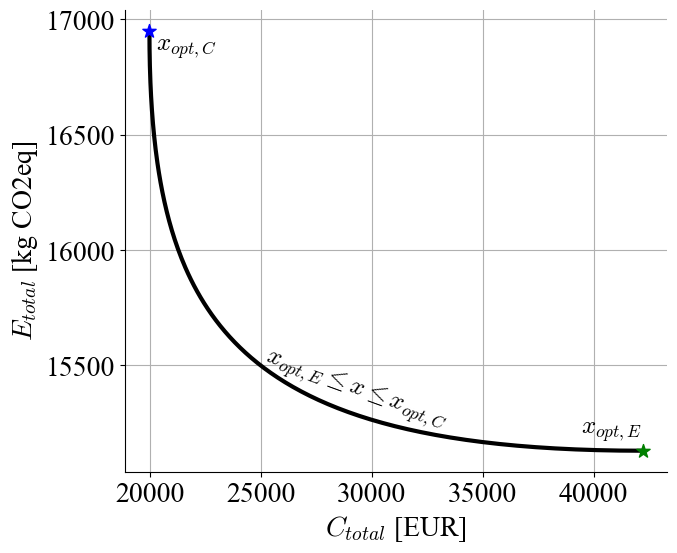
\includegraphics[width=0.7\textwidth]{Images/demo_pareto.png}
    \caption{Pareto front of the two objectives.}
    \label{fig:pareto}
\end{figure}

\subsection{Weighted sum approach / shadow costing}

The two objectives are combined into a single, augmented cost function using a shadow price $c_e$ of 0.8 euros per kilogram of CO\textsubscript{2}-equivalent emissions, which corresponds with values found in current literature \citep{EuropeanInvestmentBank2025ShadowPricing, KamaliSaraji2024BridgingApplications, Wang2017TheIndustry,  WorldBank2025PriceDashboard}.
As mentioned, this value is difficult to quantify, so the effect of different shadow prices will be investigated in the next section.

Figure \ref{fig:single} presents the single-objective optimisation, and Table \ref{tab:single} contains the numerical results, along with those from Table \ref{tab:separate} for comparison.
For a shadow cost of 0.8 \EUR{}/kg CO\textsubscript{2}eq, the optimal reliability index reduces by 0.12 with respect to the monetary optimum.
Comparing these results to the target reliability values given in ISO2394 (Table G.4) \citep{iso2394}, buildings of this consequence with `medium relative safety costs' have a target reliability of 4.2, with `small' costs increasing it to 4.4.
The monetary optimum $\beta_{opt,C}$ lies in between these two values, while the augmented optimum $\beta_{opt,aug}$ is slightly smaller than the medium value.
Therefore, for a shadow cost of 0.8 $\EUR{}$/kg CO\textsubscript{2}eq, the optimal reliability changes by `one half cost class.'


\begin{figure}[h!]
    \centering
    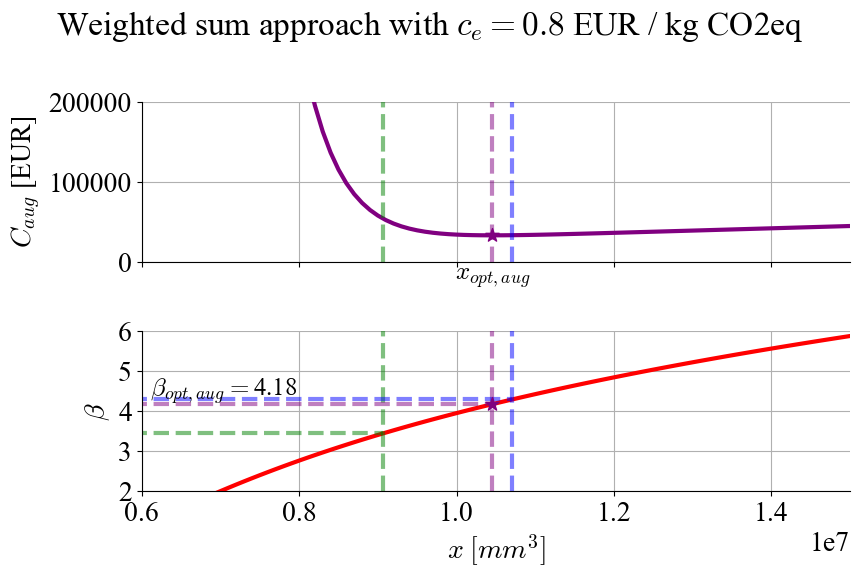
\includegraphics[width=0.85\textwidth]{Images/demo_single.png}
    \caption{Single-objective optimisation of the augmented cost function. The locations of the separate optima are indicated by dashed lines; blue for $\beta_{opt,C}$, green for $\beta_{opt,E}$, purple for $\beta_{opt,aug}$.}
    \label{fig:single}
\end{figure}

\begin{table}[]
    \centering
    \begin{tabular}{c|c|c|c}
         &   $C_{tot}$ optimal&$E_{tot}$ optimal &$C_{aug}$ optimal\\ \hline
         $x$& 
     $1.07*10^7$&$9.06*10^6$
&$1.05*10^{7}$\\
 $C_{tot}$& 19,966&42,213
&20,100\\
 $E_{tot}$& 16,951&15,129
&16,578\\
 $C_{aug}$& 33,527& 54,316&33,362\\
 $P_f$& $8.7*10^{-6}$&$2.8*10^{-4}$
&$1.5*10^{-5}$\\
 $\beta_{opt}$& 4.30&3.45&4.18\\\end{tabular}
    \caption{Results of the separate optimisation of the two objective functions}
    \label{tab:single}
\end{table}

\newpage
\subsection{$\varepsilon$-constraint approach}

As mentioned, the shadow price $c_e$ is not the only option to derive a single optimum from the two objective functions; either one can also be formulated as a constraint to the other.
To formulate the threshold values of these constraints, $E_{max}$ and $C_{max}$, the monetary optimum is considered as a reference point.
A relative desired reduction in emissions $\delta E_{desired}$ or an allowed relative increase in costs $\delta C_{allowed}$ is mandated with respect to this reference.
The problem is then formulated as:
\begin{equation}
    \begin{aligned}
        \min_{x} \quad & C_{total}(x)\\
        \textrm{s.t.} \quad & E_{total}(x) \leq E_{max} = (1 - \delta E_{desired}) \cdot E_{total}(x_{opt,C}) \\
    \end{aligned}
\end{equation}
Or:
\begin{equation}
    \begin{aligned}
        \min_{x} \quad & E_{total}(x)\\
        \textrm{s.t.} \quad & C_{total}(x) \leq C_{max} = (1 + \delta C_{desired}) \cdot C_{total}(x_{opt,C})\\
    \end{aligned}
\end{equation}
Figure \ref{fig:constrain} contains the results of this alternative approach, for different relative decreases in emissions and increases in costs.
The minimum of $E_{tot}$ is approximately 11\% smaller than the emissions at $x_{opt,C}$ (see Table \ref{tab:separate}), so this is the upper bound of $\delta E_{desired}$.
Similarly, a $\delta C_{allowed}$ up to 111\% is considered. 
In general, increasing $\delta E_{desired}$ or $\delta C_{allowed}$ decreases the constrained optimal reliability index.
For $\beta_{copt,Emax}$, this decrease appears linear for small  $\delta E_{desired}$, but becomes sharper for larger values. 
For $\beta_{copt,Cmax}$, an opposite pattern appears: the decrease is sharp for small allowed cost increases, but levels off for larger values.
This corresponds to the aforementioned shape of the separate functions in Figure \ref{fig:separate}, now connected to the reliability index: the more emissions are reduced, the more expensive reducing them becomes, \emph{as does the reduction in the optimal reliability index}.

\begin{figure}[h!]
    \centering
    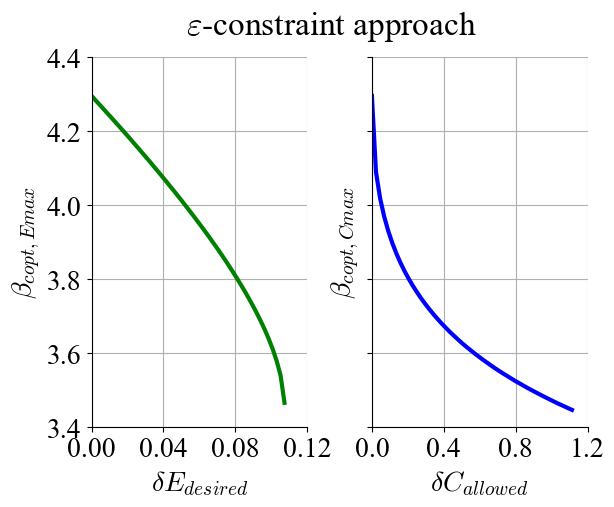
\includegraphics[width=0.6\textwidth]{Images/demo_constraint.png}
    \caption{Optimal reliability found through the $\varepsilon$-constraint approach, varying with relative contraint thresholds}
    \label{fig:constrain}
\end{figure}

% \begin{table}
%     \centering
%     \begin{tabular}{c|c|c|c|c}
%  & \multicolumn{4}{c}{$\delta E_{desired}$ w.r.t. monetary optimum}\\ \hline
%          &  0\%&  1\%&  5\%&  10\% \\ \hline
%          $x$&  $1.07*10^7$&  $1.06*10^7$&  $1.01*10^7$&  $9.37*10^6$\\
%          $C_{tot}$&  19,966&  19,990&  20,921&  30,262 \\
%          $E_{tot}$&  16,951&  16,781&  16,103&  15,256\\
%          $P_f$&  $8.7*10^{-6}$&  $1.1*10^{-5}$&  $3.0*10^{-5}$&  $1.5*10^{-4}$\\
%          $\beta_{copt,Emax}$&  4.30&  4.24&  4.01&  3.62\\
%     \end{tabular}
%     \caption{Results of optimising the cost function with a relative reduction in emissions as constraint}
%     \label{tab:E_constr}
% \end{table}


% \begin{table}
%     \centering
%     \begin{tabular}{c|c|c|c|c|c}
%  & \multicolumn{5}{c}{$\delta C_{allowed}$ w.r.t. monetary optimum}\\ \hline
%          &  0\%&  1\%&  5\%&  10\%& 20\%\\ \hline
%          $x$&  $1.07*10^7$
% &  $1.04*10^7$&  $1.01*10^7$&  $9.93*10^6$& $8.71*10^6$\\
%          $C_{tot}$&  19,966
% &  20,165&  20,962&  21,961& 23,958\\
%          $E_{tot}$&  16,951
% &  16,506&  16,090&  15,848& 15,585\\
%          $P_f$&  $8.7*10^{-6}$
% &  $1.6*10^{-5}$&  $3.1*10^{-5}$&  $4.5*10^{-5}$& $7.1*10^{-5}$\\
%          $\beta_{copt,Cmax} $&  4.30&  4.15&  4.01&  3.92& 3.81\\
%     \end{tabular}
%     \caption{Results of optimising the emission function with a relative increase in costs as constraint}
%     \label{tab:C_constr}
% \end{table}


